\documentclass{mcmthesis}
\usepackage{palatino}
\usepackage{lipsum}
\usepackage{booktabs}
\usepackage{tabu}%%table
\usepackage{colortbl}
\usepackage{indentfirst}%%suojin
\usepackage{geometry}%页面设置  
\usepackage{graphics}%图片设置  
\usepackage{caption}%注释设置  
\usepackage{graphicx}
\usepackage{subfigure}
\usepackage{palatino}
\usepackage{tikz}
\usepackage{enumerate}
\usepackage{longtable}
\usepackage{wrapfig}
\usetikzlibrary{shapes.geometric, arrows,chains}
% 设置颜色代号
\colorlet{lcfree}{green}
\colorlet{lcnorm}{blue}
\colorlet{lccong}{red}
% -------------------------------------------------
% 设置调试标志层
\pgfdeclarelayer{marx}
\pgfsetlayers{main,marx}
% 标记坐标点的宏定义。交换下面两个定义关闭。
\providecommand{\cmark}[2][]{%
  \begin{pgfonlayer}{marx}
    \node [nmark] at (c#2#1) {#2};
  \end{pgfonlayer}{marx}
  } 
\providecommand{\cmark}[2][]{\relax} 
\newcommand{\upcite}[1]{\textsuperscript{\textsuperscript{\cite{#1}}}}

%%----------------------paper------------------start------------------------------------%%
\mcmsetup{
		CTeX = false,
        tcn = 69377,
        problem = C,
        sheet = true, 
        titleinsheet = true, 
        keywordsinsheet = true,
        titlepage = false, 
        abstract = false
}


\title{Charitable Funds Boost University Education}
 %正文摘要和控制页摘要名字修改
\def\abstractname{Abstract}
\def\sheetsummaryname{summary}

\begin{document}

 %控制页摘要内容
\begin{sheetsummary}
wqeqweqweqw
\par In order to find the optimal strategy of investments, we define return on investment(ROI) based on an evaluation standard of universities' performance, introduce the investment risk to restrict target of investment, establish a Single-target Mixed Integer Linear Model with the goal of comprehensive ROI.

\par Firstly, we analyze the data by integrity and redundancy of the information, after discarding the tags and universities which are lack of data, fill out other missing data using Linear trend method.

\par Secondly, by correlating the remaining indicators based on Pearson correlation coefficient
, we categorize the indicators and select four main indicators that we believe are most relevant to evaluating school performance: graduation rates, the ability of graduates to work, retention rates, and education improvement rates. Then determine the contribution of different indicators to performance through entropy method, and calculate the performance of candidate schools, based on which, we acquire the possible value of performance of future four years through GM(1,1).

\par Finally, we use the performance change (the ratio of the mean and the variance of performance) as the investment risk, define the ROI by the performance and the annual total investment, develop a Single-target Mixed Integer Linear Programming. The optimal model is solved based on the investment risk, the total investment, and the number of investment objectives.

\par We acquire an optimal strategy and a candidate schools’ list by this Model. Take Trinity Baptist College as an example, the investment amount in the following five years is 2683937 \$, 2683937 \$, 0 \$, 2340678 \$, 2474686 \$.

\end{sheetsummary}

 %正文摘要内容
\begin{abstract}
\end{abstract}

 %关键词
\begin{keywords}
GM(1,1); Correlation Analysis; Portfolio Theory; Single-target Linear;    
\end{keywords}

\maketitle
 % Generate the Table of Contents, if it's needed.
\tableofcontents
\newpage

%%---------------------------introduction--------------------------------
\section{Introduction}


\subsection{Background}

\par In the United States, foundations are an important force in philanthropy. Many foundations, in order to promote the development of education in the United States, donate large sums of money to some schools in order to improve the education level of their schools. This kind of investment doesn’t require money returns but is based on the performance of schools. As a result, many foundations Before investing, will assess the comprehensive strength of each school, collect the data available from the school to analyze its performance, and use the return on investment as a measure of the overall strength of schools. Based on this background, this thesis designs an optimal investment strategy for Goodgrant Foundation, and give a 1 to N optimized and prioritized candidate list of schools from the best strategy.

\subsection{Our Works}

\begin{itemize}
	\item \textbf{Construct an ROI evaluation criteria}

	\par In investment economics, the main factor to measure the quality of investment is the rate of return on investment. The rate of return on investment to be considered for investment in a charitable institution is not an ordinary monetary reward. Rather, it considers the performance of a school as an investment return. Therefore, the ratio between the school performance and investment amount is the return on investment.School performance is mainly determined by indicators such as graduation rate, working ability of graduates, improvement rate of school education, and retention rate, which reflect the comprehensive strength of schools. the overall comprehensive strength of a school can be judged by judging the level of return on investment,So we decide whether to invest.
	
	
	\item \textbf{Identified the risk of investment in education}
	
	\par As the indicators describing school performance are sparsely populated, a 50\% error in the function of curve-fit performance as a function of investment will result in a much lower accuracy of the results. The use of gray prediction can be a good solution to the shortcomings of this small data. Predicting the long-term ROI by analyzing the previous data, to a certain extent, ensures the data integrity and accuracy, and provides analyzable data for solving the single-objective optimization equations later.
	
	\item \textbf{Using Grey Prediction to determine the long-term investment strategy}	
	
	\par Because of the risks of investment, in order to avoid the investment risk and make the loss of investment within the controllable range, the variance and mean ratio of the index value of each school performance for nearly four years is defined as the investment risk coefficient. From the size of the investment risk coefficient can determine the stability of the comprehensive ability of the school, so as to make the least risk investment.

		
\end{itemize}


%%--------------------------assumptions-------------------------------
\section{Assumptions}

\subsection{About the Given Data}

\begin{itemize}
	\item The data given is true and reliable, and the deletion rate is limited.
	\item Filled data can reflect the real situation.
\end{itemize}

\subsection{About Our Model}

\begin{itemize}
	\item Abandon schools with data loss rates in excess of 50\%.
	\item The local optimal solution represents the global relative solution.
\end{itemize}

%%--------------------------Analysis problem-----------------------------

\section{Analysis of the Problem}

The best investment strategies for the Goodgrant Foundation are designed to meet the requirements of the title. Among the investment strategies, there are several factors that need to be considered: the choice of schools, the investment amount of each school, the return on investment, and the investment time to motivate student performance , In order to obtain the highest comprehensive return on investment, and give a 1 to N optimized and prioritized candidate list of schools from the best strategy.

\subsection{Basic data preprocessing}

\par We found that there was a large amount of missing data by looking at the data given and the databases from both sites. Prepare the data preprocessing plan is as follows:

\begin{enumerate}[step: 1]
	\item  Discard data from schools that have data loss rates in excess of 50\%.
	\item For the remaining school data, use the linear trend method to fill.
	\item  Normalize the target variable.
\end{enumerate}

\subsection{Solution Steps}

\par We accomplish the task in several steps:
\begin{enumerate}[step 1:]
\item Determine the data items included in the school's performance index through relevancy analysis and interviews.
\item The data items to be normalized, and the use of entropy method to calculate the weight of data items.
\item Determine the ROI calculation method.
\item Define the volatility of the school performance index as a funding risk.
\item The data items to be normalized, and the use of entropy method to calculate the weight of data items.
\item Identify the schools invested and the corresponding amounts of funding through a Single- target Mixed Integer Linear Programming.
\item Calculate funding plans for the next five years by GM(1,1) forecasting data for the next five years
\end{enumerate}


\section{Symbol Description}

\begin{table}[h]
\centering
\caption{Symbol Description In This Paper}
\label{tab:Symbol Description}
\begin{tabular}{cc}
\toprule
Symbols & Description\\
\midrule
$ROI$ & return on investment\\
$X_i$ & $i$th school indicator\\
$GR$ &  Graduation rate\\
$GWA$ &  Graduates working ability\\
$EIR$ &  Education improvement rate\\
$R$ &  Retention rate\\
$SAT$ &  Average admission score\\
$R1$, $R2$, $R3$, $R4$& The retention rate of students of different years in a year\\
$R$ & The average retention rate of a student\\
$IM$ & Indicator matrix\\
$Q_m$ & investment risk factor for the m th school\\
$Q_{max}$ & Acceptable maximum investment risk factor\\
$TROI$ & Composite return on investment\\
$Q$ & The fluctuation for School Performance Index\\

\bottomrule
\end{tabular}
\end{table}


%%---------------------model-----------------------------------
\section{Establishment of the Model}

\subsection{Define ROI indicator}
Since investing needs to take into account the potential of a school to capitalize on its resources and return on investment, the school's existing rate of return on investment is required to assess the school's potential for capital utilization and to anticipate the ROI as a reference when investing in charities standard. The ROI(Return on Investment) is now given as follow:

\begin{equation}
	\label{ROI Def}
	ROI = \frac{School \quad Performance}{School \quad Income}
\end{equation}

\subsubsection{School performance index}

\par  performance represents the achievement of the school's funds and funds for school construction, access to information shows that the target results include School graduation rate increase, the ability of graduates to work, education to improve the rate of retention of students and other major indicators.Due to it has given 140 school indicators, we need to screen out the main indicators, so we use the bivariate Pearson correlation to analysis the indicators’ correlation given by the school data.

\subsubsection{Pearson correlation coefficient}

\par Using the Pearson correlation coefficient that reflects the correlation between the two variables to measure the correlation between the indicators, the Pearson correlation coefficient between every two indicators of the school is:

\begin{equation}
	\label{eq2}
	\rho_{x_{n-1},x_{n}}=corr(x_{n-1},x_n)=\frac{cov(x_{n-1},x_n)}{\sigma_{x_{n-1}}\sigma_{x_n}}
\end{equation}

Covariance($cov(x_{n-1},x_n)$) is :

\begin{equation}
	\label{eq4}
	cov(x_{n-1},x_n)=\frac{\sum \limits ^m_{i=1}(x_i-\overline{x})}{m-1}
\end{equation}

$m$ stands for school number, $\sigma_{x_{n-1}}$ and $\sigma_{x_{n}}$ is the standard deviation of the $n-1$th and $n$th indicators.


Combined with Pearson correlation coefficient and SPSS statistics, the correlation between each index is as following table \ref{tab:Correlation analysis of variables in a given data table}:
 	
\begin{table}[h]
\centering
\caption{Correlation analysis of variables in a given data table}
\label{tab:Correlation analysis of variables in a given data table}
\begin{tabular}{cccccc}
\toprule
 & SAT\_AVG\_ALL &	RET\_FT4 & gt\_25k\_p6	& PCTPELL\\
\midrule
SAT\_AVG\_ALL & - &0.155 & 0.418 & -0.549\\
RET\_FT4 & 0.155 & - & 0.148 & -0.128\\
gt\_25k\_p6 & 0.418 & 0.148 & - & -0.582\\
PCTPELL & -0.549 & -0.128 & -5.82 & - \\

\bottomrule
\end{tabular}
\end{table}

This table shows the correlation between the performance-related indicators and the performance-related indicators that we determined based on the relevant information. Since indicators with very little relevance can show the performance of different aspects of the school, The paper chooses the composition of the indicators that have the lowest relevancy and is closely related to the school's performance as the main indicators. We have chosen the following indicators.

\subsubsection{Select indicators}

We have chosen the following indicators according to above method.

\begin{enumerate}
	\item \textbf{graduation rate (GR)}: 
	
		Graduation rate includes 3 variables: GBA4RTT, GBA5RTT, and GBA6RTT. We use the final 6-year graduation rate(GBA6RTT) as GR.
		
	\item \textbf{Graduates' ability to work}:
	
		Students' ability to work(GWA) is determined by the ratio of student winners(it's CSTOTLT in access data base) to total school attendance(it's UGDS in access data base).

		\begin{equation}
			\label{GWA}
				GWA \quad = \frac{CSTOTLT}{UGDS}			
		\end{equation} 
	

	\item \textbf{The rate of increase in education(EIR)}:
		 The ratio of post-graduate ability to pre-admission ability. The improvement of education is reflected in the improvement of students' abilities. Therefore, the average admission score (SAT) of all students before enrollment is selected as the pre-admission ability, and the award rate is used as a reflection of GWA after graduation.
		 
		 \begin{equation}
		 	\label{EIR}
		 		EIR = \frac{GWA}{SAT}
		 \end{equation}

	\item \textbf{retention rate (R)}: 
		The actual number of students reported in a class and the ratio of the number of theoretical reports. The retention rates R1, R2, R3, R4(it's RET\_FT4, RET\_FTL4, RET\_PT4, RET\_PTL4 in access data base) for the four different types of students given in the school data are averaged to give a retention rate R.
		\begin{equation}
			\label{R}
				R = \frac{R1+R2+R3+R4}{4}			
		\end{equation}
\end{enumerate}

\subsubsection{Entropy Method to Determine Performance}
\par Principle of Entropy Method: Entropy is a concept derived from thermodynamics. In 1948, Shannon introduced the information entropy for the first time to describe the uncertainty of the signal source, which is a measure of the order of the system. The smaller the entropy of evaluation index, indicating that the greater the degree of variation of the index value, the greater the amount of information provided, the greater the weight. And because of the subjectivity of AHP in determining the weight of index value, this model uses information entropy to determine the objective weight of each index according to the degree of variation of each index value.
\begin{itemize}
	\item Citing the values of the four main indicators (GR, GWA, EIR, R) in the data processing, the indicator matrix (IM):
		\begin{equation}
		\label{eq6}
		IM=(q_{im})_{4\times m}=\left(\begin{array}{cccc}
		q_{1,1} & q_{1,2} & \ldots & q_{1,m}\\
		q_{2,1} & q_{2,2} & \ldots & q_{2,m}\\
		q_{3,1} & q_{3,2} & \ldots & q_{3,m}\\
		q_{4,1} & q_{4,2} & \ldots & q_{4,m}\\
		\end{array} \right)
		\end{equation}
		
		$m$ represents the number of schools,  $q_{i,m} \quad (i = 1,2,3,4)$ followed by four indicators (GR, GWA, EIR, R).
	\item Give the entropy definition. The four indicators (GR, GWA, EIR, R) in the indicator matrix correspond in turn to their entropy $e_i \quad (i=1,2,3,4)$.
 
	
		\begin{equation}
		\label{eq8}
		\left\{
			\begin{aligned}
				&e_i & = \quad & -k\sum^m_{j=1}Z_{ij}ln(Z_{ij}) \\
				&z_{i,j} & = \quad & \frac{q_{ij}}{\sum\limits ^m_{j=1}q_{ij}} \\
				&k & = \quad & \frac {1}{ln(m)}
			\end{aligned}
		\right.
	\end{equation}

	$k$, $z_{i,j}$ is an intermediate variable. When $z_{i,j}$ will result in logarithmic meaningless, so that $z_{ij}\cdot ln z_{i,j}$.
	\item Define entropy weights. According to the definition of entropy, four indicators (GR, GWA, EIR, R) in the indicator matrix correspond to their entropy $\omega_i \quad i = 1,2,3,4$.

		\begin{equation}
			\label{eq10}
			\left\{
			\begin{split}
				&\omega_i & = \quad & \frac{1-e_i}{4-\sum\limits^4_{i=1}e_i} \\
				&\sum^4_{i=1}\omega_i & = \quad & 1 \\
				&k & = \quad & \frac {1}{ln(m)}
			\end{split}
			\right.
		\end{equation}

		Combined with equation \ref{eq6},\ref{eq8},\ref{eq10}, we can find that the weights of the four indicators (GR, GWA, EIR, R) as follow.
		\begin{equation}
			\label{eq11}
			\omega_1=0.2501 \quad \omega_2=0.2501 \quad \omega_3=0.2496 \quad \omega_4=0.2501
		\end{equation}
	
\end{itemize}


\subsubsection{School income index}

We choose the school's total annual income as the school income index. For three kinds of schools, we choose the following data for School income index:

\begin{itemize}
	\item \textbf{Public institutions}: Total operating and noperating revenues
	\item \textbf{Private not-for-profit institutions}: Total revenues and investment return
	\item \textbf{Private for-profit institutions}: Total revenues and investment return
\end{itemize}

\subsubsection{ROI formula}
According to the definition of $ROI_m$ formula give its specific formula.

\begin{equation}
	\label{eq17}
	ROI_m = \frac{SP_m}{SI_m} = \frac{0.2501\cdot GR + 0.2501\cdot GWA + 0.2501\cdot EIR +0.2496\cdot R}{Total\quad operating\quad and\quad noperating\quad revenues}
\end{equation}

$SI_m$ Is the $m$th school's income, $SP_m$ is the $m$th school's performance. 

\subsection{ROI forecast for the next five years}

\par Based on the ROI data for each of the four previous schools for each of the four years, GM(1, 1) forecasts the ROI of each school in the next five years.

\subsubsection{GM(1,1)}

\par The traditional GM (1,1) model\upcite{gm} is composed of a differential equation containing univariate.
\par Let $X^{(0)}=[x^{(0)}(1), x^{(0)}(2),\cdots ,x^{(0)}(n)]$ , $X^{(1)}=[x^{(1)}(1), x^{(1)}(2),\cdots ,x^{(1)}(n)]$ , $Z^{(1)}=[z^{(1)}(1), z^{(1)}(2),\cdots ,z^{(1)}(n)]$ , where $x^{(1)}(k) =  \sum\limits_{i=1}^k x^{(1)}(i)$ and $z^{(1)}(k) = \frac{x^{(0)}(k) + x^{(0)}(k+1)}{2}$ , then $x^{(0)}(k) + a z^{(1)}(k) = b$ is called the GM(1,1) model. The parameter $a$ is called the development coefficient, and the parameters $b$ is called the grey action quantity.
 
Then, we can get the time responded function of GM(1,1) model.
\begin{equation}
\hat{x}^{(1)}(k+1) = (x^{(0)}(1) - \frac{b}{a})e^{-a k} + \frac{b}{a} \qquad k = 1, 2, \cdots, n
\end{equation}
and the restored function of $x^{(0)}(k + 1)$ can be given by

\begin{equation}
\hat{x}^{(0)}(k+1) = (1 - e^a)(x^{(0)}(1) - \frac{b}{a})e^{-a k} \qquad k = 1, 2, \cdots, n
\end{equation}

\par In which, $\hat{x}^{(1)}(k)$ is the simulative value of  $x^{(1)}(k)$, and  $\hat{x}^{(0)}(k)$ is simulative value of $x^{(0)}(k)$

\par Without external interference, we know that the population and GDP was exponential growth. But this model will produce a continuously simulative deviation when simulating a homogeneous-exponent sequence. Because the unequal conversion between the discrete difference equation and continuous differential equation. So we learn from C.I.Chen\upcite{}. The Discrete GM(1,1) Model as follows:
\begin{equation}
\hat{x}^{(1)}(k+1) = (x^{(0)}(1) - \frac{b}{a})(\frac{2 - a}{2 + a})^k+ \frac{b}{a} \qquad k = 1, 2, \cdots, n
\end{equation}
\begin{equation}
\hat{x}^{(0)}(k+1) = (1 - \frac{2 + a}{2 - a})(x^{(0)}(1) - \frac{b}{a})(\frac{2 - a}{2 + a})^k \qquad k = 1, 2, \cdots, n
\end{equation}
\par Use least squares to solve $a$ and $b$. Put it into the prediction formula. We can get the predictive value $X^{(1)}$, and the analog value of $X^{(0)}$.\\




\subsection{Definition of Risk}

\par In financial sector, Modern Portfolio Theory was used to measure risk and benefits, drawing the Efficient Frontier of all the risky assets and find the Tangency Portfolio\upcite{PT}.  For charitable investment, there also exists risk, which will forbid investment reaching the optimal point though it does not bring any lost for you. Here we define “risk” fo our investment.
	\begin{equation}
		\label{risk}
		Q = \frac{S^2_e}{\mu_e}
	\end{equation}
\par In the formula, we use the concept of coefficient of variation. $S^2_e$ indicates the variance of School Performance Index, and $\mu_e$ indicates the means of School Performance Index. 

\subsection{Establish a single objective optimization equation\upcite{single}}

\par The primary school for philanthropic investment focuses on the strength of schools and the potential for capital utilization to maximize the return on comprehensive investment. The standard for quantifying the strength of schools and capitalizing their potential is the return on investment (ROI) for each school over the next four years, To establish a single-objective optimization equation that takes the total investment return (TROI) as the target and the investment amount $\omega_m$ as the variable.

\begin{equation}
	\label{eq20}
	TROI=\sum\limits^{n}_{m=1}ROI_m\cdot \omega_m
\end{equation}

\par $m$ represents the $m$th school, the total number is $n$; $ROI_m$for the first m schools return on investment,  those have been GM (1,1) predicted. In order to solve this equation, the following constraints are given as follows:
\begin{enumerate}[(1)]
	\item To not exceed the total annual investment amount A, give the investment amount constraint:

\begin{equation}
	\label{eq22}
	\left\{
	\begin{split}
	&A & = \quad & 100000000\$ \\
	&m\cdot \omega_m & = \quad & A \\
	&\omega_m &\leqslant \quad & A
\end{split}
\right.
\end{equation}

\par $A$ is the total investment of 100 million US dollars.
	\item As the number of schools invested by charitable organizations can not be infinite, and to maximize the return on investment, the number of selected schools needs to be limited to select the best investment schools. So given the number of school restrictions.

\begin{equation}
	\label{eq29}
	10\leqslant m \leqslant 50
\end{equation}

\par The final single-objective optimization equation for total ROI is as follows:

\begin{equation}
	\label{eq30a}
	TROI = \sum\limits^{n}_{m=1}ROI_m\cdot\omega_m
\end{equation}
 
\begin{equation}
	\label{eq30b}
	\left\{
	\begin{split}
	& m \cdot\omega_m & = \quad &A\\
	&\omega_m & \leqslant \quad & A\\ 
	&\sum\limits^{n}_{m=1}Q_m\cdot\omega_m &\leqslant \quad &A\cdot Q_{max}\\
	&10 &\leqslant\quad & m &\leqslant\quad & 50
\end{split}
\right.
\end{equation}


                            
\par $m$ represents the $m$th school, the total number is $n$; TROI is the comprehensive return on investment, $ROI_m,\omega_m,Q_m,Q_{max}$ is the m school return on investment, $ROI_m,\omega_m,Q_m,Q_{max}$ is the first m of the school's investment amount, A total amount of 100 million, $ROI_m,\omega_m,Q_m,Q_{max}$is To describe the ratio of the volatility of investment risk, $ROI_m,\omega_m,Q_m,Q_{max}$ is the maximum risk factor the organization can bear.

\end{enumerate}



\section{Calculation and Analysis of the Model}

\subsection{Data preprocessing\upcite{data1,data2}}

\begin{enumerate}
	\item Eliminate schools with data loss rates above 50\%, given the missing information on the various indicators given for each school.
	\item Exclude schools under the supervision of the Ministry of Education, cannot be awarded a bachelor's degree.
	\item Using a regression equation was used to fill in the missing values with the missing values 
	\item Since each index unit is not uniform, its data are normalized so as to obtain complete and analyzable data with a total of 572 schools' data.
\end{enumerate}


\subsection{Basic ROI Calculation}

This gives a return on investment of 572 schools. Specific results are as following table \ref{tab:Past 4 Years ROI Calculation Results} :

\begin{table}[h]
\centering
\caption{Past 4 Years ROI Calculation Results}
\label{tab:Past 4 Years ROI Calculation Results}
\begin{tabular}{cccccc}
\toprule
unit ID & Institution Name & 2013 & 2014 & 2015 & 2016 \\
\midrule
448840	&University of South Florida-St Petersburg	&35.81	&43.71	&41.11	&45.28\\
433660	&Florida Gulf Coast University &	 14.85 & 16.34 & 16.52 & 14.80\\
392840	&Watkins College of Art Design  Film & 240.20	& 371.51 & 332.42 & 478.11\\
366711	&California State University-San Marcos	& 19.32	& 19.76 & 20.99 & 16.11\\
243780	&Purdue University-Main Campus &	2.12	 & 2.06	&2.37	& 2.41\\
240727	&University of Wyoming &	5.73 &	6.13 &	 7.39	& 6.07\\
240480	&University of Wisconsin-Stevens Point	&17.64	&18.40	&22.74	&20.94\\
240471	&University of Wisconsin-River Falls	 & 29.98 & 	32.10 &	40.12 &	33.90\\
240462	&University of Wisconsin-Platteville	 & 24.44 &	24.87 &	25.55 &	22.40\\
$\cdots$&$\cdots$&$\cdots$&$\cdots$&$\cdots$&$\cdots$\\
\bottomrule
\end{tabular}
\end{table}

\newpage

\par The ROI values in the above table \ref{tab:Past 4 Years ROI Calculation Results} are accurate to two decimal places, sorted from high to low, giving the ROI of some schools. According to the ROI of each school, the potential and the investment value of the school can be judged.

\par The estimated ROI of 572 schools for the next five years is shown in the following table \ref{tab:Next 5 Years ROI Predict Results}.
\begin{table}[h]
\centering
\caption{Next 5 Years ROI Predict Results}
\label{tab:Next 5 Years ROI Predict Results}
\begin{tabular}{cccccc}
\toprule
Institution Name & 2017 & 2018 & 2019 & 2020 & 2021\\
\midrule
University of South Florida-St Petersburg	&45.00	&45.85	&46.71	&47.58	&48.48\\
Florida Gulf Coast University	&14.43	&13.76	&13.12	&12.51	&11.93\\
Watkins College of Art Design \& Film	&522.31	&604.57	&699.78	&809.99	&937.56\\
California State University-San Marcos	&15.74	&14.37	&13.12	&11.98	&10.93\\
Purdue University-Main Campus	&2.64	&2.85	&3.07	&3.30	&3.56\\
University of Wyoming	&6.48	&6.46	&6.43	&6.41	&6.38\\
University of Wisconsin-Stevens Point	&23.22	&24.62	&26.10	&27.66	&29.33\\
University of Wisconsin-River Falls	&37.09	&37.98	&38.89	&39.83	&40.78\\
University of Wisconsin-Platteville	&21.96	&20.90	&19.89	&18.93	&18.02\\
$\cdots$&$\cdots$&$\cdots$&$\cdots$&$\cdots$&$\cdots$\\
\bottomrule
\end{tabular}
\end{table}

\par Due to the large number of schools, this table has only selected some of the schools to display. From the above table, it can be initially seen that the ROI of some schools shows an increase while some of them have Therefore, when re-investing, we not only need to use the annual ROI as a reference standard, but also pay attention to the volatility of the ROI to reduce the investment risk.


\subsection{Solve Single-target Mixed Integer Linear Programming}
\subsubsection{Solve Best Investment Strategy for First Year}

\par Now equation \ref{eq30a}, \ref{eq30b} for the single objective optimization equation, we solve the Fmincom function to Predict the school to be invested for first year, the amount of investment, and the maximum ROI. We use the median of all school risks as the risk threshold which is $Q_{max} = 0.00064011$.  The result are as following table \ref{tab:First Best Investment Advice Form} (In order to show more data in this table, we expend the risk $Q$ for 1000 times).

\begin{table}[h]
\centering
\caption{First Best Investment Advice Form}
\label{tab:First Best Investment Advice Form}
\begin{tabular}{cccccc}
\toprule
unit ID &	 Institution Name &	ROI & Risk	& Investment\\
\midrule
176789 &	Calvary Bible College and Theological Seminary	&1061.75&	3.18	&806756\\
137953&	Trinity Baptist College	&644.85	&0.39	 &2683937\\
392840&	Watkins College of Art Design  \& Film	 &451.24&	7.47 &0\\
224244&	Dallas Christian College	&412.83	&3.38	 &3113685\\
169327&	Cleary University	&408.07	&0.11 	&3645894\\
102669&	Alaska Pacific University	&306.54	&11.76	&3231178\\
204176&	Mount Carmel College of Nursing & 	289.44	&8.25	 &2521678\\
219198&	Mount Marty College	&277.79	&1.68 	&2409603\\
117104&	Life Pacific College&	266.21&	14.23&	2340678\\

$\cdots$&$\cdots$&$\cdots$&$\cdots$&$\cdots$\\
\bottomrule
\end{tabular}
\end{table}

\par In the above table \ref{tab:First Best Investment Advice Form}, the ROI is accurate to two decimal places. Risk is the investment risk coefficient, and Investment is the investment amount. From the investment risk coefficient, most investment schools have a low investment risk coefficient and a few investment risk factors are high Schools, because of their high rate of return on investment, so there are also involved in investment. Therefore, investment risk and return on investment are the two major criteria for investment.

\par The proportion of investment in each school is now shown in figure \ref{50 Schools Funded by the Amount Allocate}.

\begin{figure}[!h]
\small
\centering
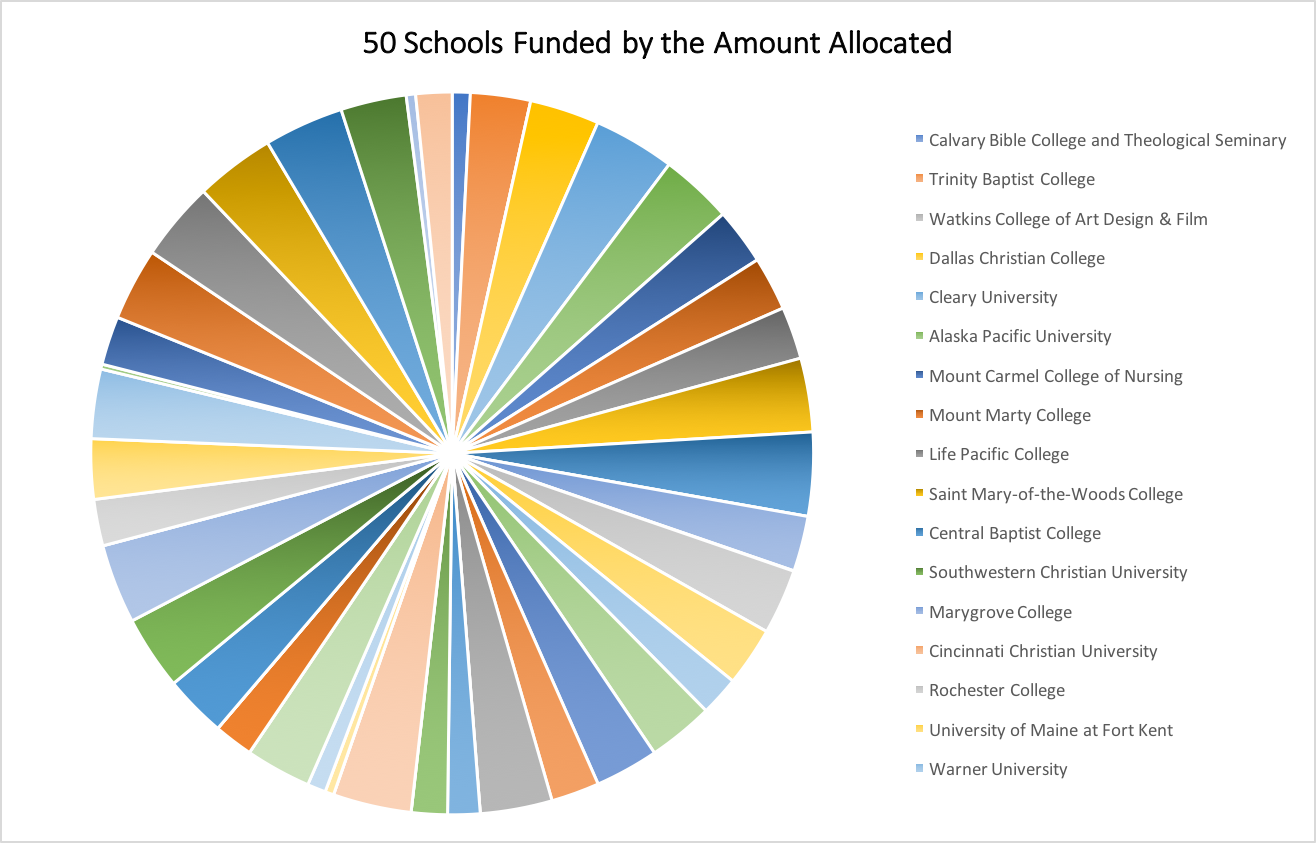
\includegraphics[width=14cm]{year1_part.png}
\caption{50 Schools Funded by the Amount Allocate} \label{50 Schools Funded by the Amount Allocate}
\end{figure}

\par For the picture above, each one represents the investment amount of each school, it has 50 schools and a total investment of 100 million US dollars. As can be seen from the figure, the distribution of funds is relatively average. Combining the investment objectives of charitable organizations, we can see that in order to improve the education level in more schools, we need to allocate resources more evenly so that the results are consistent with their purpose.

\subsubsection{The Optimal Investment Strategy for the Next Four Years}

\par Assuming that the funds invested by the institution will not change each year, the same method can be used to predict the annual investment plan for next four years. Therefore, the investment plan for the next five years is given as following tables \ref{tab:Second Year's Best Investment Advice Form},\ref{tab:Third Year's Best Investment Advice Form},\ref{tab:Fourth Year's Best Investment Advice Form},\ref{tab:Fifth Year's Best Investment Advice Form} (In order to show more data in this table, we expend the risk $Q$ for 1000 times).

\begin{table}[h]
\centering
\caption{Second Year's Best Investment Advice Form}
\label{tab:Second Year's Best Investment Advice Form}
\begin{tabular}{cccccc}
\toprule
unit ID &	 Institution Name &	ROI & Risk	& Investment\\
\midrule
176789&	Calvary Bible College and Theological Seminary&	1747.04	&3.18	&806756\\
137953&	Trinity Baptist College	&556.30	&0.39	&2683937\\
392840&	Watkins College of Art Design \& Film&	522.31&	7.47&	0\\
224244&	Dallas Christian College &	433.89	&3.38&	3113685\\
169327&	Cleary University	&429.16	&0.11	&3645894\\
204176&	Mount Carmel College of Nursing	&340.02&	8.25&	3231178\\
102669&	Alaska Pacific University&	333.30&	11.76&	2521678\\
219198&	Mount Marty College	&322.17&	1.68	&2409603\\
106713&	Central Baptist College&	310.48&	2.23&	2340678\\

$\cdots$&$\cdots$&$\cdots$&$\cdots$&$\cdots$\\
\bottomrule
\end{tabular}
\end{table}


\begin{table}[h]
\centering
\caption{Third Year's Best Investment Advice Form}
\label{tab:Third Year's Best Investment Advice Form}
\begin{tabular}{cccccc}
\toprule
unit ID &	 Institution Name &	ROI & Risk	& Investment\\
\midrule
176789&	Calvary Bible College and Theological Seminary&	2874.66&	3.18&	806756\\
137953&	Trinity Baptist College&	479.91&	0.39&	0\\
392840&	Watkins College of Art Design \& Film&	604.57&	7.47&	2683937\\
224244&	Dallas Christian College&	456.03&	3.38&	3113685\\
169327&	Cleary University&	451.35&	0.11&	3645894\\
204176&	Mount Carmel College of Nursing & 	399.43 &	8.25&	3231178\\
102669&	Alaska Pacific University&	362.41&	11.76&	2340678\\
219198&	Mount Marty College&	373.64&	1.68&	2409603\\
106713&	Central Baptist College&	389.80&	2.23&	2521678\\
$\cdots$&$\cdots$&$\cdots$&$\cdots$&$\cdots$\\
\bottomrule
\end{tabular}
\end{table}

\begin{table}[h]
\centering
\caption{Fourth Year's Best Investment Advice Form}
\label{tab:Fourth Year's Best Investment Advice Form}
\begin{tabular}{cccccc}
\toprule
unit ID &	 Institution Name &	ROI & Risk	& Investment\\
\midrule
176789&	Calvary Bible College and Theological Seminary&	4730.08&	3.18&	806756\\
392840&	Watkins College of Art Design \& Film&	699.78&	7.47&	2683937\\
106713&	Central Baptist College&	489.37&	2.23&	0\\
224244&	Dallas Christian College&	479.29&	3.38&	3113685\\
169327&	Cleary University&	474.68&	0.11&	3645894\\
204176&	Mount Carmel College of Nursing&	469.22&	8.25&	3231178\\
219198&	Mount Marty College&	433.34&	1.68&	2521678\\
115728&	Holy Names University&	421.05&	23.00&	2409603\\
137953&	Trinity Baptist College&	414.00&	0.39&	2340678\\
$\cdots$&$\cdots$&$\cdots$&$\cdots$&$\cdots$\\
\bottomrule
\end{tabular}
\end{table}


\begin{table}[h]
\centering
\caption{Fifth Year's Best Investment Advice Form}
\label{tab:Fifth Year's Best Investment Advice Form}
\begin{tabular}{cccccc}
\toprule
unit ID &	 Institution Name &	ROI & Risk	& Investment\\
\midrule
176789&	Calvary Bible College and Theological Seminary&	7783.07&	3.18&	806756\\
392840&	Watkins College of Art Design \& Film&	809.99&	7.47&	2683937\\
106713&	Central Baptist College&	614.39&	2.23&	0\\
115728&	Holy Names University&	563.02&	23.00&	3113685\\
204176&	Mount Carmel College of Nursing&	551.20&	8.25&	3645894\\
200156&	University of Jamestown&	539.63&	17.60&	3231178\\
224244&	Dallas Christian College&	503.74&	3.38&	2521678\\
219198&	Mount Marty College&	502.58&	1.68&	2409603\\
169327&	Cleary University&	499.21&	0.11&	2340678\\
$\cdots$&$\cdots$&$\cdots$&$\cdots$&$\cdots$\\
\bottomrule
\end{tabular}
\end{table}



\begin{figure}[htbp]  
\begin{minipage}[t]{0.5\textwidth}
\centering  
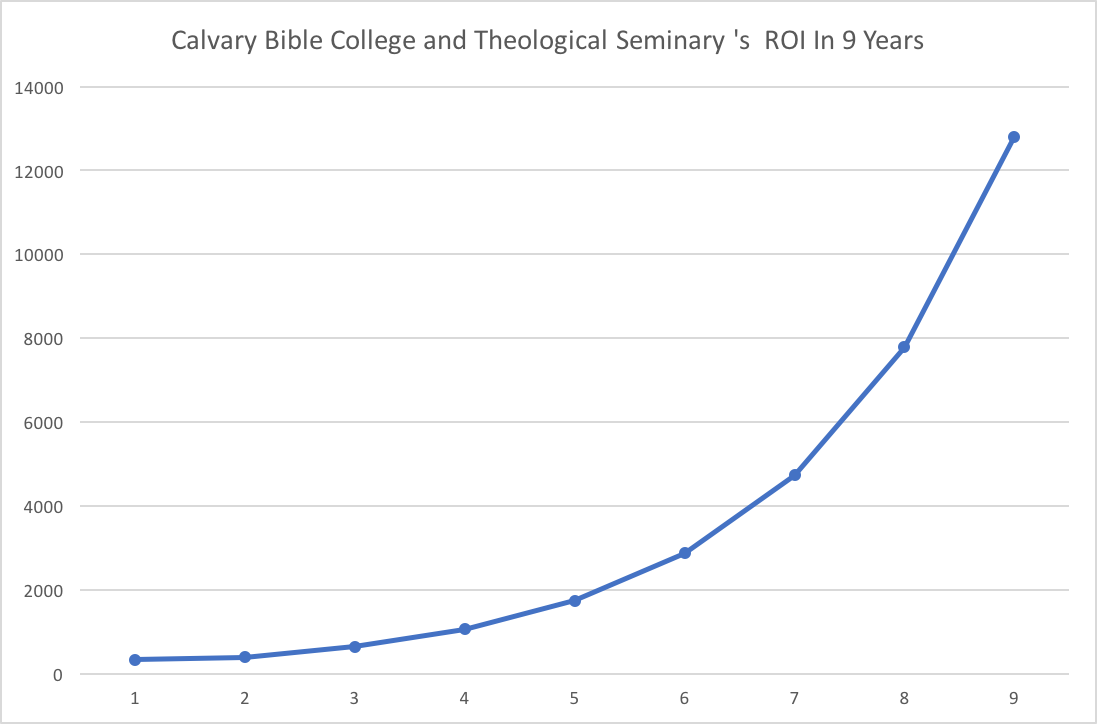
\includegraphics[width=\linewidth]{ROI_9_1.png} \\
X-axis = Years\quad Y-axis = ROI
\caption{Calvary Bible College and Theological Seminary 's  ROI In 9 Years} 
\label{Calvary Bible College and Theological Seminary 's  ROI In 9 Years}
\end{minipage}
\hspace{1ex}
\begin{minipage}[t]{0.5\textwidth}  
\centering  
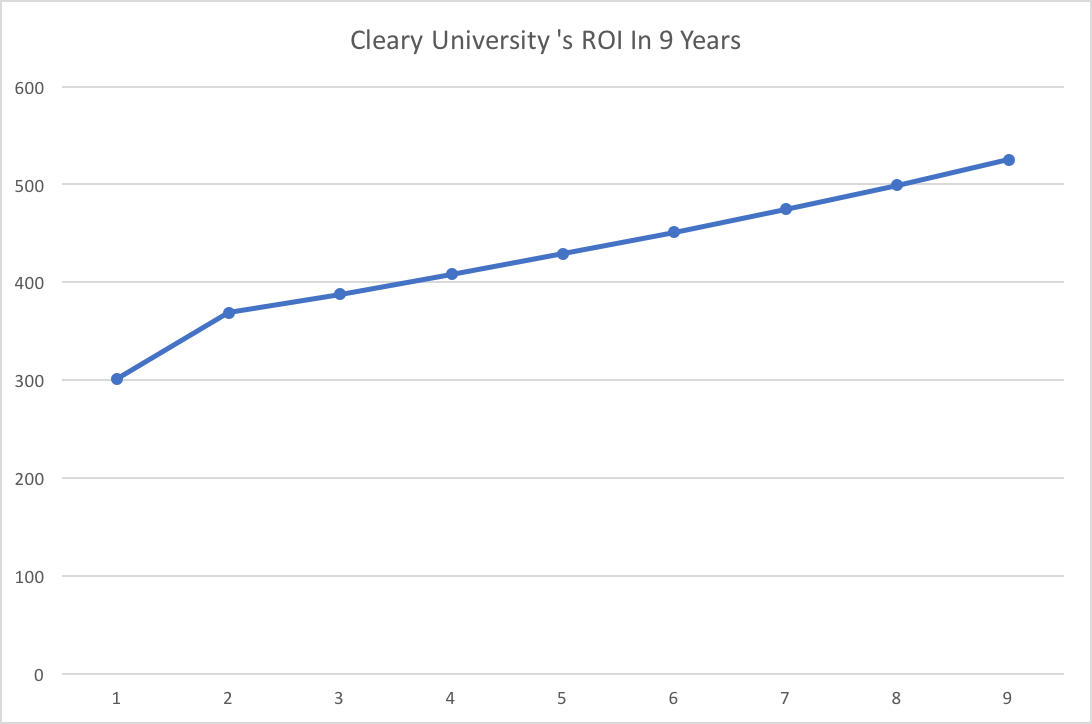
\includegraphics[width=\linewidth]{ROI_9_2.png}\\
X-axis = Years\quad Y-axis = ROI
\caption{Cleary University 's ROI In 9 Years}  \label{Cleary University 's ROI In 9 Years}
\end{minipage}  
\end{figure} 

\newpage

\par The table shows the annual investment plan for next for years. From the table, we can see that most of the schools invested each year have not changed and the risk coefficient does not fluctuate much. Therefore, we can see that Schools are constantly upgrading their education level in the continuous investment process . For specific analysis, we can choose Calvary Bible College and Theological Seminary, Cleary University for analysis.

\par As can be seen from the figure \ref{Calvary Bible College and Theological Seminary 's  ROI In 9 Years}, \ref{Cleary University 's ROI In 9 Years}, after the investment, the return on investment of College and Theological Seminary and Cleary University continues to increase. Although the rate of return on investment at Cleary University School is rising slowly, it is still increasing. By analyzing other schools, we can also find that under the investment, the ROI of most schools is constantly improving. Therefore, we can see that this investment strategy has the ability to improve school education.

\par However, not all schools have improved levels of education, as can be seen in the table \ref{tab:Some Schools Five-year Subsidy} below.

\begin{table}[h]
\centering
\caption{Some Schools Five-year Subsidy}
\label{tab:Some Schools Five-year Subsidy}
\begin{tabular}{cccccc}
\toprule
INSTNM & Year 1 & Year 2 & Year 3 & Year 4 & Year 5\\
\midrule
Trinity Baptist College & 2683937 & 2683937 & 0 & 2340678 & 2474686\\
Watkins College of Art Design \& Film & 0 & 0 & 2683937 & 2683937 & 2683937\\
Dallas Christian College & 3113684 & 3113684 & 3113684 & 3113684 & 2521677\\
Cleary University & 3645894 & 3645894 & 3645894 & 3645894 & 2340678\\
Alaska Pacific University & 3231177 & 2521677 & 2340678 & 3741025 & 3741025\\
Mount Carmel College of Nursing & 2521677 & 3231177 & 3231177 & 3231177 & 3645894\\
Mount Marty College & 2409603 & 2409603 & 2409603 & 2521677 & 2409603\\
Life Pacific College & 2340678 & 2643213 & 2936629 & 0 & 0\\
Saint Mary-of-the-Woods College & 3299144 & 3299144 & 0 & 18348 & 2917307\\
Central Baptist College & 3741025 & 2340678 & 2521677 & 0 & 0\\
Southwestern Christian University & 0 & 3217725 & 2077921 & 0 & 0\\
Marygrove College & 2474686 & 3741025 & 2474686 & 2917307 & 2643213\\
\bottomrule
\end{tabular}
\end{table}

\newpage

This table shows only some of the school's investment amount, the specific form in Appendix 1. As can be seen from the above table, schools such as Trinity Baptist College and Life Pacific College may not receive any investment after several years of investment. This may be due to an increase in the school's investment risk or no obvious improvement in education levels, resulting in Not in line with charities to maximize return on investment. Schools like Watkins College of Art Design \& Film and Southwestern Christian University, for example, They did not receive any investment from the start, but later received an investment indicating. This shows that each year this model can be adjusted according to the school's overall strength and return on investment and risk changes to give the best investment strategy.




\section{Strengths and Weaknesses}
\subsection{Strengths}
\begin{itemize} 
\item Make full use of all the data given, we use linear trend method to fill in the missing value, to ensure the accuracy of the data.

\item After reading the information, we have customized the return on investment, investment risk coefficient, etc., with a high degree of innovation.

\end{itemize}
\subsection{Weaknesses}
\begin{itemize}
	\item The direct deletion of schools with data loss rates up to 50\% may delete certain potential schools and result in some bias.
	\item Our definition of ROI does not reflect well the impact of funding itself.
\end{itemize}


\section{A letter to the Goodgrant Foundation}

Dear Sir/Madam:

\par We are honored to help you choose the best donation target. Here we will give the definition of Return on investment(ROI), explain the investment strategy and analysis method that make the ROI highest, and finally give the ROI ranking of schools from high ROI to low ROI in accordance with the best investment strategy.
\par As we know, Goodgrant Foundation's goal is to improve the education level of American colleges. Therefore, the return on investment can be measured by the level of education level in universities and the level of colleges can be measured by the performance of a school. So, in order to get the maximum return on comprehensive investment ,  we will give a definition of the performance of a school firstly.
\par Since the performance of a school reflects the school's level of education, the rate of return on investment is now defined as the ratio of school performance to school income, so we need to find indicators that reflect school performance. As for student, they pay for college and aim to enhance their ability to work. Therefore, we choose the ability of graduates to work as one of the main indicators. From a social perspective, if it is difficult for students to graduate from a school, the quality of its education level may be a poor. So the graduation rate and retention rate of students are selected as two of the main indicators. From the aspect of education, if the quality of education is improved, the teachers and students' ability to work in the school can be improved. Therefore, the rate of education improvement is selected as one of the main indicators. Thus, the four major indicators closely related to school performance are determined: graduation rate of students, education promotion rate, working ability of graduates and retention rate of students. When we read the existing indicator data that reflects school performance , we find  most of the indicator data are repetitive or meaningless. Therefore, by analyzing the correlation degree between the indicators through the correlation analysis method, we combine the indicators with high correlation and find indicators which can reflect the four main indicators above. We use the entropy method to determine the weight of each indicator and determine the investment of each school response rate according to the product of each indicator and the weight of it as .
\par We choose the ratio between the investment and the schools’ performance as the return on investment. Because not every school can effectively use the funds to improve self-education level, it is necessary for you to choose before you invest. Because the data of some schools is incomplete, some schools are under the control of the Ministry of Education and some schools do not grant undergraduate degree, the missing data of whom within 50\% data loss rate are filled in with the linear trend method and the others are removed. According to the return on investment of nearly four years in each school, we use the GM (1,1) method to predict the return on investment over the next five years. Every investment is risky, so in order to avoid the investment risk, we use the variance and mean of return on investment Ratio as the risk coefficient of investment to analyze its four-year investment risk. We assume the maximum acceptable risk coefficient is the median of the investment risk coefficient, choose the risk coefficient less than the maximum risk as a constraint, the most comprehensive return on investment  as a goal and solve the single objective optimization equation with the investment amount as the variable in order to find the optimal investment strategy.  
\par To sum up, we predict the optimal annual investment strategy for 5 years as following table \ref{tab:Some Schools Five-year Subsidy}:

\begin{table}[h]
\centering
\caption{Some Schools Five-year Subsidy}
\label{tab:Some Schools Five-year Subsidy}
\begin{tabular}{cccccc}
\toprule
INSTNM & Year 1 & Year 2 & Year 3 & Year 4 & Year 5\\
\midrule
Trinity Baptist College & 2683937 & 2683937 & 0 & 2340678 & 2474686\\
Watkins College of Art Design \& Film & 0 & 0 & 2683937 & 2683937 & 2683937\\
Dallas Christian College & 3113684 & 3113684 & 3113684 & 3113684 & 2521677\\
Cleary University & 3645894 & 3645894 & 3645894 & 3645894 & 2340678\\
Alaska Pacific University & 3231177 & 2521677 & 2340678 & 3741025 & 3741025\\
Mount Carmel College of Nursing & 2521677 & 3231177 & 3231177 & 3231177 & 3645894\\
Mount Marty College & 2409603 & 2409603 & 2409603 & 2521677 & 2409603\\
Life Pacific College & 2340678 & 2643213 & 2936629 & 0 & 0\\
Saint Mary-of-the-Woods College & 3299144 & 3299144 & 0 & 18348 & 2917307\\
Central Baptist College & 3741025 & 2340678 & 2521677 & 0 & 0\\
Southwestern Christian University & 0 & 3217725 & 2077921 & 0 & 0\\
Marygrove College & 2474686 & 3741025 & 2474686 & 2917307 & 2643213\\
$\cdots$&$\cdots$&$\cdots$&$\cdots$&$\cdots$&$\cdots$\\
\bottomrule
\end{tabular}
\end{table}





\newpage

\begin{thebibliography}{99}

\bibitem{gm} Tan G J. The Structure Method and Application of Background Value in Grey System GM(1,1) Model (Ⅰ)[J]. SYSTEMS ENGINEERING-THEORY \& PRACTICE, 2000, 20(5):125-127.
\bibitem{single} Richards A, Schouwenaars T, How J P, et al. Spacecraft Trajectory Planning with Avoidance Constraints Using Mixed-Integer Linear Programming[J]. Journal of Guidance Control \& Dynamics, 2002, 25(4):755-764.
\bibitem{corr} Hardoon D R, Szedmak S, Shawe-Taylor J. Canonical Correlation Analysis: An Overview with Application to Learning Methods[J]. Neural Computation, 2014, 16(12):2639-2664.
\bibitem{PT} In Princeton Companion to Applied Mathematics Princeton University Press. Portfolio Theory[J]. Princeton Companion to Applied Mathematics Princeton University Press.
\bibitem{data1} \url{www.nces.ed.gov/ipeds}
\bibitem{data2} \url{https://collegescorecard.ed.gov}
\end{thebibliography}








\begin{appendices}

\par 50 schools in the next 5 years the amount of funding calculation results(table \ref{tab:50 Schools Five-year Subsidy}).

\begin{table}[h]
\centering
\caption{50 Schools Five-year Subsidy}
\label{tab:50 Schools Five-year Subsidy}
\begin{tabular}{cccccc}
\toprule
INSTNM & Year 1 & Year 2 & Year 3 & Year 4 & Year 5\\
\midrule
Calvary Bible College & 806756 & 806756 & 806756 & 806756 & 806756\\
Trinity Baptist College & 2683937 & 2683937 & 0 & 2340678 & 2474686\\
Watkins College of Art Design & Film \& 0 & 0 & 2683937 & 2683937 & 2683937\\
Dallas Christian College & 3113684 & 3113684 & 3113684 & 3113684 & 2521677\\
Cleary University & 3645894 & 3645894 & 3645894 & 3645894 & 2340678\\
Alaska Pacific University & 3231177 & 2521677 & 2340678 & 3741025 & 3741025\\
Mount Carmel College of Nursing & 2521677 & 3231177 & 3231177 & 3231177 & 3645894\\
Mount Marty College & 2409603 & 2409603 & 2409603 & 2521677 & 2409603\\
Life Pacific College & 2340678 & 2643213 & 2936629 & 0 & 0\\
Saint Mary-of-the-Woods College & 3299144 & 3299144 & 0 & 18348 & 2917307\\
Central Baptist College & 3741025 & 2340678 & 2521677 & 0 & 0\\
Southwestern Christian University & 0 & 3217725 & 2077921 & 0 & 0\\
Marygrove College & 2474686 & 3741025 & 2474686 & 2917307 & 2643213\\
Cincinnati Christian University & 18348 & 2474686 & 1761951 & 2839048 & 3217725\\
Rochester College & 2917307 & 1613080 & 392573 & 2077921 & 416098\\
University of Maine at Fort Kent & 2643213 & 1761951 & 2643213 & 1761951 & 1761951\\
Warner University & 1761951 & 2157836 & 3217725 & 1443964 & 0\\
Oakland City University & 2937459 & 1443964 & 0 & 0 & 826702\\
Blackburn College & 2839048 & 2839048 & 2937459 & 2937459 & 2937459\\
Holy Names University & 2157836 & 0 & 3299144 & 2409603 & 3113684\\
Friends University & 3217725 & 2917307 & 18348 & 0 & 3299144\\
Judson University & 0 & 3507028 & 1613080 & 826702 & 0\\
University of Sioux Falls & 1443964 & 0 & 2157836 & 2157836 & 2839048\\
Erskine College & 1613080 & 0 & 3507028 & 0 & 3314292\\
University of Jamestown & 0 & 18348 & 3741025 & 3299144 & 3231177\\
Coker College & 3507028 & 2937459 & 2917307 & 2474686 & 0\\
MidAmerica Nazarene University & 0 & 0 & 3314292 & 0 & 2172278\\
Olivet College & 392573 & 826702 & 0 & 3507028 & 3507028\\
Roberts Wesleyan College & 826702 & 392573 & 1443964 & 3217725 & 1443964\\
Truett-McConnell College & 2936629 & 2936629 & 0 & 392573 & 2936629\\
Lancaster Bible College & 0 & 0 & 0 & 2172278 & 0\\
Valley City State University & 1756329 & 0 & 2172278 & 2937359 & 0\\
Toccoa Falls College & 0 & 3314292 & 3102160 & 3250179 & 1621848\\
Union College & 0 & 217316 & 0 & 0 & 0\\
Bluefield State College & 2780508 & 0 & 2839048 & 2643213 & 18348\\
Malone University & 3314292 & 1756329 & 826702 & 2936629 & 392573\\
Bethel College-Indiana & 3553563 & 0 & 0 & 0 & 0\\
Spalding University & 0 & 2780508 & 2780508 & 0 & 2780508\\
Northwest University & 2077921 & 3102160 & 217316 & 217316 & 217316\\
Ohio Dominican University & 2689672 & 3553563 & 0 & 0 & 0\\
Wilmington College & 3102160 & 2172278 & 3250179 & 3516047 & 3552950\\
Missouri Baptist University & 217316 & 416098 & 0 & 0 & 0\\
Siena Heights University & 2172278 & 3560335 & 0 & 0 & 0\\
Concordia University-Texas & 3250179 & 3552950 & 0 & 0 & 0\\
Paine College & 3516047 & 2077921 & 1756329 & 1613080 & 0\\
Holy Family University & 3552950 & 3250179 & 2689672 & 2780508 & 3553563\\
Concordia University-Portland & 3560335 & 2689672 & 0 & 0 & 2157836\\
Lakeland College & 2937359 & 2937359 & 1621848 & 416098 & 3560335\\
Howard Payne University & 416098 & 0 & 0 & 0 & 0\\
Geneva College & 1621848 & 1621848 & 2937359 & 3552950 & 3102160\\
\bottomrule
\end{tabular}
\end{table}

\end{appendices}

\end{document}

